
\documentclass[11pt]{article} % Loads settings for the document layout

\usepackage{geometry}
 \geometry{
 a4paper,
 total={210mm,297mm},
 left=25mm,
 right=25mm,
 top=25mm,
 bottom=25mm,
 }
\usepackage{setspace}
 \doublespacing
 
\usepackage{gensymb}

\usepackage{graphicx}

\usepackage{subfigure}

\usepackage{float}
% Preamble

% The following settings are used for title generation and will show up in the
% main document where the \maketitle command is set.
\title{DSC424 - Group 1: Final Project Report}
\date{\today}
\author{Isabelle Na Young Choi, Stephanie Olivera, Milad Sabouri, \\
Chien-Lin Yang \& Pengju Zhang}

% Main document

\begin{document} % The document starts here

\maketitle % Creates the titlepage

\pagenumbering{arabic} % Turns on page numbering

\noindent\rule{\linewidth}{\arrayrulewidth}

\section*{Project Summary}
In this project, we investigated Marketing Data\cite{githubLink} to analyze a marketing campaign. The dataset includes a variety of information about customers like education, income, marital status, children, amount of money spent on different products, and customers' responses on campaigns. Also, the data shows us how customers have done their purchases through different means. The dataset includes 2,240 samples of customers behaviors in the last 2 years that have been featured by 28 variables. In this project, by analyzing customers' behaviors in the past, we want to see whether they will respond to a future marketing campaign. 

\noindent\rule{\linewidth}{\arrayrulewidth}

\clearpage
\tableofcontents
\noindent\rule{\linewidth}{\arrayrulewidth}

\newpage
\section{Non-Technical Summary}
\subsection{Data Exploratory}
We understand all variables in the data and find relationships between variables so that it is helpful to find better analysis. Several preprocessing actions were applied to the marketing data in an effort to identify variables which were missing a number of values. New variables are created by merging some variables and dividing into groups. The initial regression is one of data exploratory analysis processes which is to show relationships between variables and find strong correlation between variables. And visualization can show an interesting relationship between some features. It can help to show more clearly the relationship between variables then help to find a better method of analysis. 
\subsection{Regression Analysis}
We developed multiple regression models to try to predict the total number of purchases made by a given customer. Our first goal was to determine which subset of features are most important for predicting the total number of purchases a customer will make. Our second goal was to create a model with high predictive power. We found that the following features were most significant for predicting the total number of purchases: income, number of kids at home, amount spent on wines, amount spent on fruits, amount spent on meat products, amount spent on gold products  and whether the customer accepted the 5th marketing campaign. Additionally, we found that customers with kids at home and customers that accepted campaign 5 tend to purchase less items. 
\subsection{Principal Component Analysis}
We tried to understand the most significant variables in the data by performing principal component analysis. We found out that a household that has more children at home probably has more web visits per month. It might be because young people do like to shop through online platforms. Also, by increasing the age of customers the number of complaints will increase. Moreover, the analysis shows us that income has an impact on total number of purchases and total amount of purchases while by increasing the number of children the total amount of purchase items may decrease.
\subsection{Linear Discriminant Analysis}
In addition, we also try to use LDA to analyze the data. Based on customer profiles, products purchased, consumption habits, we want to predict whether they will accept the marketing campaign, and further explore whether we can predict the income level of customers based on their consumption habits data. We can further explore the possibility of targeting different promotions to customers in different income levels. Our prediction result can reach 70\%-80\%, which is a good result. Therefore, we can use LDA to provide the sales department with the related analysis results, such as what type of spending style people are in what income level.
\subsection{Cluster Analysis}
Finally, we implement clustering analysis to distinguish each group more visually. We perform both general and reduced dimension dataset (PCA) for clustering analysis, both reports tells us that a grouping of 2 or 3 classes is the best optimal choice, and by using the histogram for analyzing the whole data, we get the pattern that income has the best fit, by manually giving it a label and re-plotting it on the existing chart (with 2 clusters), we can get overall 80\% fit, as the result, we confirm that our clustering results have a high correlation with income.

\newpage
\section{Technical Summary}
\subsection{Data Exploratory}
\quad The original data set contained over 2240 observations and 28 variables. According to the preprocessing phase of the project, new 5 variables were added to valuable for the modeling phase. There are new 5 variables which is a total amount variable, total number of purchase variable, total children variable, age class variable, and income class variable. Total amount variable was merged some amount of product spent that is MntWines, MntFruits, MntMeatProducts, MntFishProducts, MntSweetProducts, MntGoldProds. There are 3 variables which are included in NumWebPurchases, NumCatalogPurchases, and NumStorePurchase is presented number of purchases made through various pathway. These variables were merged as a total number of purchase variable.  Both Kidhome and Teenhome variables were showing a number of minorities in customer’s household so that these were merged a total children variable.  Also, age and income variables were widely used in a variable so that it needed to create a class. An age class variable divided into customer group based on their age which is baby boomers, X-generation, millennials, and Z-generation.  An income class variable also formed an income group which included in the rich, upper-middle, middle, lower-middle, and poor. 

\quad Initial regression is helped to determine strengths of relationship between variables before analysis. The first initial regression can show a relationship some variables, age, income, total children, recency, and amount of money spent on different products. As you can see the figure 1, The F-test looks good, so we are rejecting the null hypothesis and accepting the alternative that at least one is not equal to zero. The adjusted R-squared is that 71.04\% of the variability in Y is explained by the model. Most t-test look good except the total\_children and recency variables. I can reject that null hypothesis and accept the alternative that they are not equal to zero. Another initial regression is using campaign variables. The figure 2 can show the f-test looks good, and T-test also looks good that all p-values are less than 0.005. I can reject the null hypothesis and accept the alternative. However, the R-squared and the adjusted R-squared is quite low which is 19.5\%. 
\begin{figure}[H]
    \centering
    \subfigure[]{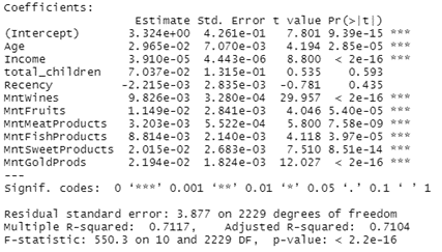
\includegraphics[width=0.5\textwidth]{Isabelle/i-t-1.png}}
    \subfigure[]{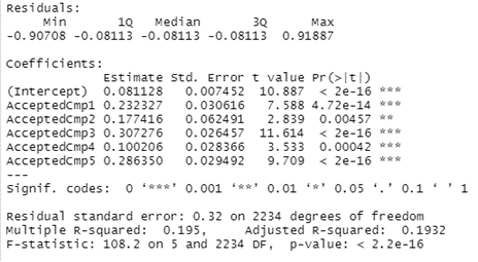
\includegraphics[width=0.5\textwidth]{Isabelle/i-t-2.png}} 
    \caption{t-test}
    \label{fig:foobar}
\end{figure}

\quad Final data exploratory is visualizing relationships between the variables in the marketing dataset. There are 3 visualization features to show interesting relationships between variables and to help to find relationships between low potential target features. First figure a represented numeric versus numeric features. The correlation matrix is to represent all numeric features in the data. Some correlations are strong especially income and products purchased variables. These have strong correlation with the total amount of purchases. Next figure b is categorical versus numeric features. These boxplots show relationship between the total amount of purchased feature and the categorical features, which is income class, marital status, age class, country, complain, and response. The last figure c shows categorical versus categorical features. These multiple mosaic plots represent the relationship between the response feature and the categorical features which is age, marital status, education, and country. 
\begin{figure}
    \centering
    \subfigure[]{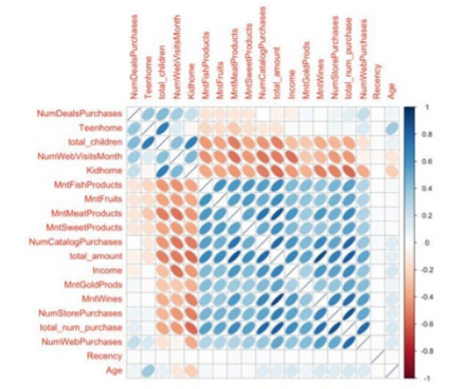
\includegraphics[width=0.5\textwidth]{Isabelle/i-t-3.png}}
    \subfigure[]{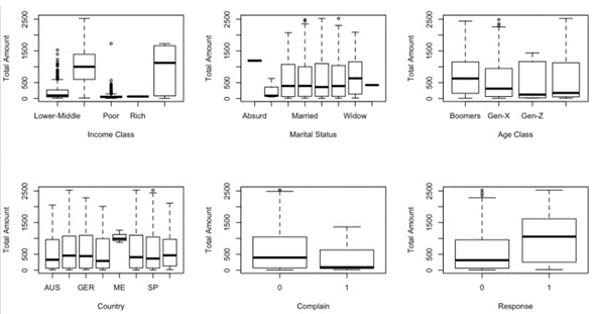
\includegraphics[width=0.5\textwidth]{Isabelle/i-t-4.png}} 
    \subfigure[]{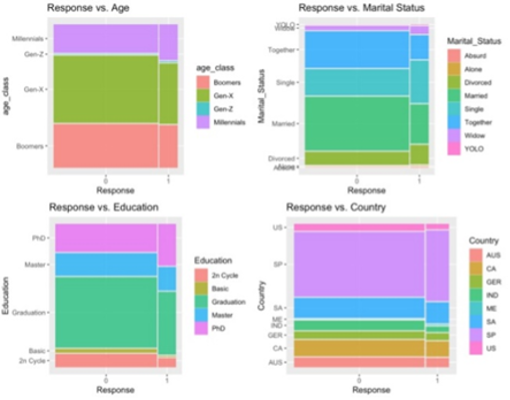
\includegraphics[width=0.5\textwidth]{Isabelle/i-t-5.png}} 
    \caption{(a): Scatter plots (b): Box plots (c): Mosaic Plots}
    \label{fig:foobar}
\end{figure}
\newpage
\subsection{Regression Analysis}

\quad For our first line of analysis we chose to do a regression analysis with the total number of purchases as our parameter of interest. We started off by creating an OLS regression model with all features. Here, we found that many of the parameters were not significant, with t-test p-values greater than .05. We decided to proceed with all-subsets regression to find the best set of features for predicting the total number of purchases. The results of our all-subsets regression are shown in Fig. 1a. Here we can see that the following 8 features are significant for predicting total number of purchases: Income, Kidhome, MntWines, MntFruits, MntMeatProducts, MntSweetProducts, MntGoldProducts and AcceptedCampaign5. We then proceeded to create a regression model using only the 8 significant features selected by all-subsets. The resulting betas are shown in Fig. 1b. Here, we can see that the largest coefficients are AcceptedCmp5 and KidHome with high negative values.
\begin{figure}[H]
    \centering
    \subfigure[]{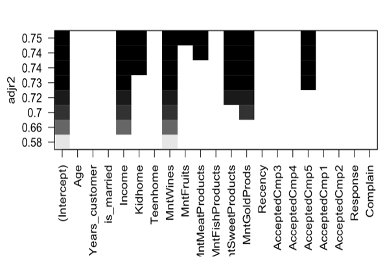
\includegraphics[width=0.4\textwidth]{Stephanie/s-t-1.png}}
    \subfigure[]{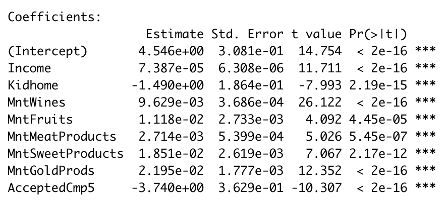
\includegraphics[width=0.4\textwidth]{Stephanie/s-t-2.png}} 
    \caption{(a): Figure a (b): Figure b}
    \label{fig:foobar}
\end{figure}

\quad To evaluate the predictive performance of this model, we fit the linear regression model above using a 90\% train set. We then evaluated the model by first making predictions on the train set to obtain the train RMSE with a value of 3.65. Next, we obtained the test RMSE by using the model to make predictions on the 10\% test set and obtained a value of 4.71. Here, the model is performing much better at predicting the total number of purchases for samples in the train set than in the test set. This is a strong indication of overfitting, which suggests potential to improve our predictive performance on the test set by using regularized regression techniques.

\quad Next, we proceeded with Lasso regression to attempt to combat overfitting and to have an independent approach for feature selection to compare to our results from all-subsets selection. Using the 9\% train set, we first performed 10-fold cross validation to find the optimal value of lambda. The resulting plot is shown in Fig. 2a. We decided to select the lambda 1se value to create a more parsimonious model with only 10 features. The features selected by our Lasso regression model were Income, Kidhome, Teenhome, MntWines, MntFruits, MntMeatProducts, MntFishProducts, MntSweetProducts, MntGoldProducts and AcceptedCampaign5. To evaluate this model, we calculated the train RMSE and test RMSE using the same procedure as above and obtained a train RMSE of 3.73 and test RMSE 4.71. Here, we can see that the train and test RMSE values are getting closer together, but there is still room for improvement.
\begin{figure}[H]
    \centering
    \subfigure[]{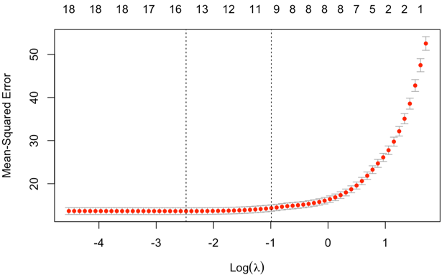
\includegraphics[width=0.4\textwidth]{Stephanie/s-t-3.png}}
    \subfigure[]{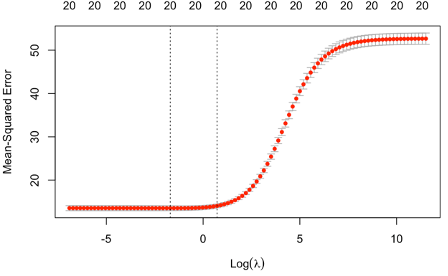
\includegraphics[width=0.4\textwidth]{Stephanie/s-t-4.png}} 
    \caption{(a): Figure a (b): Figure b}
    \label{fig:foobar}
\end{figure}
\quad Next, we chose to create a ridge regression model to see if we could further improve the predictive performance of the model. We again used 10-fold cross validation to find the optimal value for the lambda regularization parameter and chose the lambda-1se value shown in Fig. 2b. Next, we calculated the train RMSE and test RMSE with values of 3.705 and 4.37. Here we can see that the ridge regression model is performing much better at predicting total number of purchases than both the all-subsets and lasso regression models.

\quad Finally, as suggested by the professor, we decided to proceed with elastic net regression to combine the predictive power of ridge regression and the feature selection capabilities of lasso regression. Here, we found that setting the alpha parameter of glmnet() to 0.5 which mixes 50\% Lasso and 50\% Ridge gave the best results. The model selected the same 10 features as our Lasso regression model with one additional feature, Years\_customer. With values of 3.68 and 4.53, both our train RMSE and test RMSE improved compared to Lasso. 

\quad With a test RMSE of 4.37, our ridge regression model had the best predictive performance. However, the elastic net model is also a great choice because it is a more parsimonious model with a slightly higher test RMSE of 4.53. Additionally, we found the the following features were all considered significant in All-Subsets, Lasso and elastic net feature selection: Income, Kidhome, MntWines, MntFruits, MntMeatProducts, MntSweetProducts, MntGoldProducts and AcceptedCampaign5. Finally, we found that in all regression models, KidHome and AcceptedCampaign5 had the highest negative beta values while TeenHome was the only feature with a large positive beta value. 

\subsection{Principal Component Analysis}

\quad To find the relation between different variables in this project, we performed several principal component analysis. Overally, we applied PCA techniques over 22 variables. According to the initial correlation plot we realized that four, five, or maybe 6 components are significant among variables. To find the best number of components, we initiated a simple PCA and we applied four different techniques including scree plot, var=1, cumulative proportion, and parallel analysis. 

\begin{figure}[H]
    \centering
    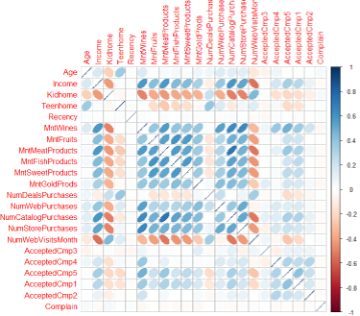
\includegraphics[width=0.5\textwidth]{Maild/m-t2-1.png}
    \caption{Figure a}
    \label{fig:foobar}
\end{figure}

\quad According to the knee on scree plot and parallel analysis the good number of components are four. However, based on var=1 and cumulative proportion techniques the good number of components should be six. So, we decided to investigate both numbers and compare the outcomes. According to the results, if we choose 6 to be the number of factors, we will have some components that only one variable has a contribution to them. On the other hand, by choosing 4 as the number of components, the result is not something that we can interpret in a meaningful way. 

\begin{figure}[H]
    \centering
    \subfigure[]{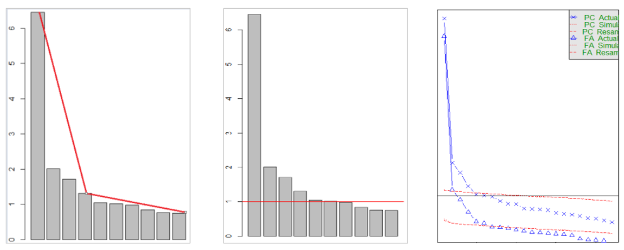
\includegraphics[width=0.7\textwidth]{Maild/m-t2-2.png}}
    \subfigure[]{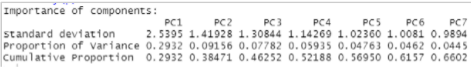
\includegraphics[width=0.7\textwidth]{Maild/m-t2-3.png}} 
    \caption{(a): Figure a (b): Figure b}
    \label{fig:foobar}
\end{figure}

\quad Since our goal is to find the most significant principal components in order to build a parsimonious model, we decided to perform further analysis on data. To do that, we use corr.test function to find the variables that have no correlation with others and also, find variables that have correlations with almost all other variables. Based on the result of factor cleaning, we found out that there are two variables that have no correlations with others. Also, there are four variables that have correlation with more than 80\% of other variables. By considering these two facts, we applied a second PCA on the data. based on the four techniques of finding the good number of components, we found that 5 is an appropriate number of factors. We performed different PCA analysis by setting the number of factors as 5. We run both principal functional and factanal functions. We tried to look for some consensus among the results. For the second analysis, we realized interpreting the results is quite challenging. In addition, there were some factors that only one variable had a contribution to. At this point, we decided to perform more analyses on the data, by merging some variables and creating new variables. In fact, in the original data there are two variables called KidHome (number of customer’s kids at home) and TeenHome (number of customer's teens at home). We thought that it is better to merge these two variables to one variable. So, we created a new variable called total\_children which is the sum of KidHome and TeenHome. Also, the original dataset includes six variables that indicate the number of amounts that each customer has purchased in six products (Wines, Fruits, Meat, Fish, Sweets, Gold). We created one new variable called total\_amount which is the sum of these six products. Furthermore, the original dataset includes information about how customers have purchased products in the past. There are three ways to purchase products: 1) Purchasing through online websites; 2) Purchasing by using catalogs; 3) Purchasing on physical stores. The dataset includes the number of times that each customer has purchased products in each of these three ways. We created a new variable called total\_num\_purchased which is a sum of the total number of purchases that each customer has had using a website, store, or catalog. This new variable may help us to have a straightforward analysis on total purchase for each customer. After that, we performed our third PCA analysis on the data. Again we applied four different techniques to find the best number of factors. According to the results of these four techniques, we realized that 3 should be an appropriate number for choosing significant components. In fact, by selecting the first three components we can have almost 60\% of data. We can say that we have three components that we named them: 
\begin{enumerate}
    \item Income
    \item Children
    \item Age
\end{enumerate}
The following are the formulas that show the contributor of each component: 
\begin{enumerate}
    \item \textbf{RC1 (Income)} = .807*Income - .568*NumWebVisitsMonth – .429*total\_children + .914*total\_amount + .897*total\_num\_purchases + .506*total\_acceptance
    \item \textbf{RC2 (Children)} = .898*NumDealPurchases + .501*NumWebVisitMonths + \\ .680*total\_children
    \item \textbf{RC3 (Age)} = .620*Age + .473*Recency + .544*Complain
\end{enumerate}

\quad According to the results, income, the total amount of purchases, the total number of purchased items, and the total number of acceptance of previous campaigns have positive contributions to the first factor which we name Income because it has the most significant contributor of this factor. However, the number of web visits per month and the total number of children at home have negative contributions to the first factor. On the other hand, the number of web visits and total children at home has positive contributions to the second factor which we named Children. The contributors of the third factor are age, recency, and complaint. We named the third factor Age. The first factor (Income) shows us that income has an impact on the total number of purchases and the total amount of purchases while by increasing the number of children the total amount of purchase items may decrease. The Second factor (Children) shows us that households that have more children are more towards online shopping. It is because young people may like shopping in this way. Also, young people most like to shop for products that have discount deals. The third factor (Age) shows us that by increasing the age probably the number of complaints will increase as well.
\subsection{Linear Discriminant Analysis}

\quad Linear discriminant analysis is used as a tool for classification, dimension reduction, and data visualization. In our marketing data, we want to predict whether customers will accept the marketing campaign, and the dependent variable is binary (yes/ no). We use logistic regression to compare with LDA and find that the prediction accuracy of both is similar by the confusion matrix and ROC curve.
\begin{figure}[H]
    \centering
    \subfigure[]{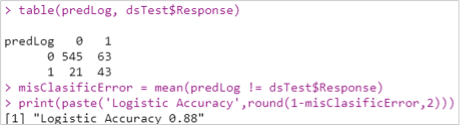
\includegraphics[width=0.4\textwidth]{Chien-Lin/c-t-1.png}}
    \subfigure[]{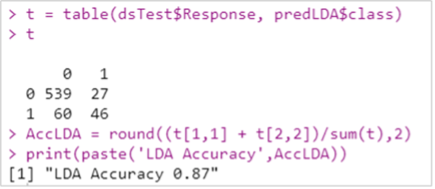
\includegraphics[width=0.4\textwidth]{Chien-Lin/c-t-2.png}} 
    \subfigure[]{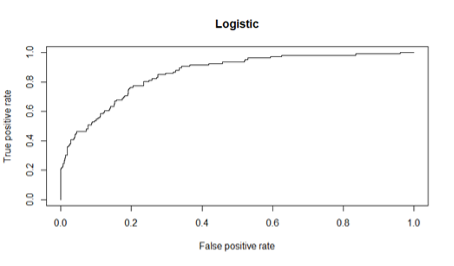
\includegraphics[width=0.4\textwidth]{Chien-Lin/c-t-3.png}}
    \subfigure[]{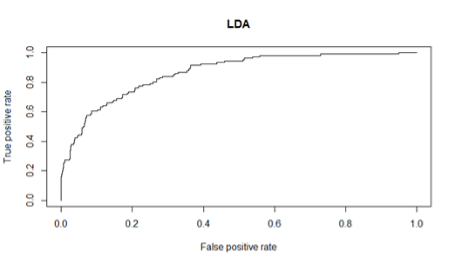
\includegraphics[width=0.4\textwidth]{Chien-Lin/c-t-4.png}} 
    \caption{(a): Logistic Result  (b): LDA Result (c): Logistic Plot (d): LDA Plot}
    \label{fig:foobar}
\end{figure}

\quad In addition to understanding whether customers would accept the marketing campaign, we also want to find out if the consumer behavior and style could classify different income levels so that we could further target people in different income levels with an efficient approach to do different modes of a marketing campaign. We use "income\_class" as the dependent variable, which has five levels: Poor, Lower-Middle, Middle, Upper-Middle, and Rich. The independent variables are different shopping styles, such as discount purchasing, catalog purchasing, store purchasing, and website purchasing. The initial model is difficult to see the classification of income levels, and the prediction accuracy is not good. Therefore, we try to improve the problem in two parts: adjust the classification of income levels to make it clearer and remove a relatively insignificant variable in LD1. Then, we find that the income level classification is still not easy to read, but the prediction accuracy becomes better.
\begin{figure}[H]
    \centering
    \subfigure[]{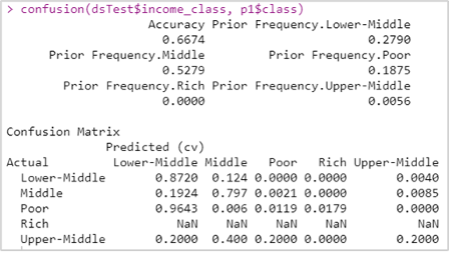
\includegraphics[width=0.4\textwidth]{Chien-Lin/c-t-5.png}}
    \subfigure[]{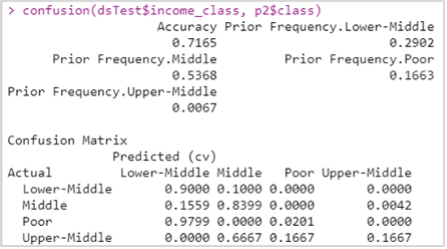
\includegraphics[width=0.4\textwidth]{Chien-Lin/c-t-6.png}} 
    \subfigure[]{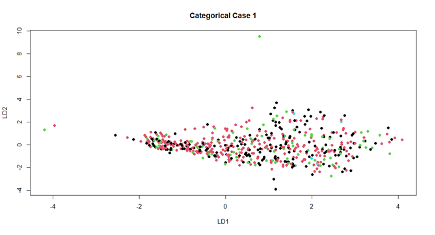
\includegraphics[width=0.4\textwidth]{Chien-Lin/c-t-7.png}}
    \subfigure[]{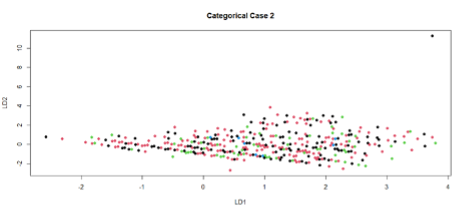
\includegraphics[width=0.4\textwidth]{Chien-Lin/c-t-8.png}} 
    \caption{(a): Result Before  (b): Result After (c): Plot Before (d): Plot After}
    \label{fig:foobar}
\end{figure}
\subsection{Cluster Analysis}

\quad Classification as a supervised learning method requires that the information of each category must be explicitly known in advance and that all items to be classified are asserted to have a category corresponding to them. However, many times the above conditions are not satisfied, especially when dealing with large amounts of data, and it is very costly to make the data satisfy the requirements of the classification algorithm by preprocessing, so clustering can be considered. In contrast, clustering does not rely on training instances with predefined classes and class labels.

\quad When we look at certain data sources, it is likely that we will find the data clusters in some form. For example, in our data, the distribution of residents' incomes are distributed in two categories, one above the average and the other below. 

\begin{figure}[H]
    \centering
    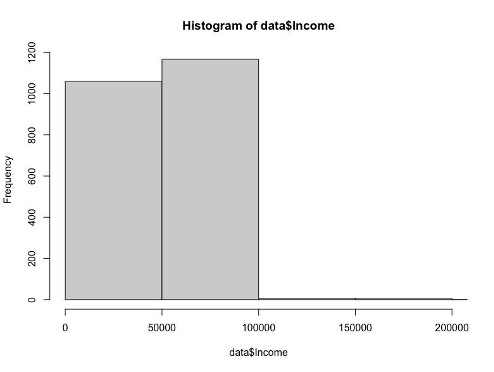
\includegraphics[width=0.5\textwidth]{Pengju/p-t-1.jpg}
    \caption{Income Histogram}
    \label{fig:foobar}
\end{figure}

\quad There are two factors that have a great impact on clustering analysis, one is the number of optimal clusters, another one is the algorithm for clusters. In our dataset, we perform elbow method, silhouette method and dendrogram to confirm our final optimal clusters.

\begin{figure}[H]
    \centering
    \subfigure[]{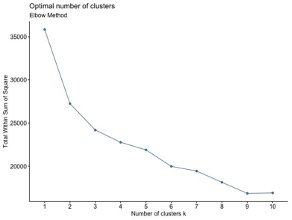
\includegraphics[width=0.4\textwidth]{Pengju/p-t-2.jpg}}
    \subfigure[]{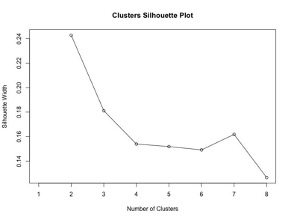
\includegraphics[width=0.4\textwidth]{Pengju/p-t-3.jpg}} 
    \subfigure[]{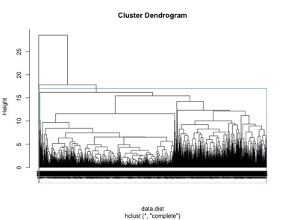
\includegraphics[width=0.4\textwidth]{Pengju/p-t-4.jpg}}
    \caption{(a): Elbow Method  (b): Silhouette Method (c): Dendrogram}
    \label{fig:foobar}
\end{figure}

\quad Elbow graph has a sharp elbow downwards at the 2nd and 3rd point, the rest of them equally contribute to the same error to the total variance, this indicates the optimal number of 3 as a good cluster. For the dendrogram, it is roughly separated by 2 main parts, left and right below the height of 15. Finally the highest value of Silhouette width indicates the number of 2 as an optimal cluster.

\begin{figure}[H]
    \centering
    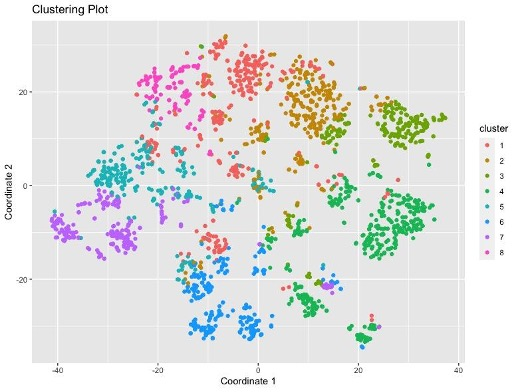
\includegraphics[width=0.5\textwidth]{Pengju/p-t-5.jpg}
    \caption{Lower Dimension Clustering}
    \label{fig:foobar}
\end{figure}

\quad In order to clearly see the pattern in our dataset, we try to plot all clusters from 1 to 8 in lower dimension with less random data, but most of them cross with each other.

\begin{figure}[H]
    \centering
    \subfigure[]{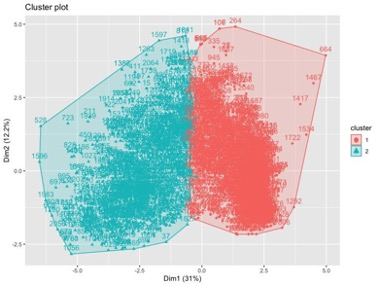
\includegraphics[width=0.4\textwidth]{Pengju/p-t-6.jpg}}
    \subfigure[]{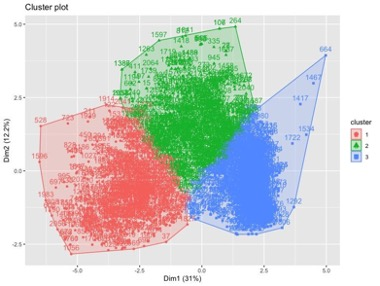
\includegraphics[width=0.4\textwidth]{Pengju/p-t-7.jpg}} 
    \caption{(a): Cluster of 2  (b): Cluster of 3}
    \label{fig:foobar}
\end{figure}

\quad By applying the k-means algorithm for our clustering, as far as we can see, they do have very clear separation for both graphs, but the central area is too messy to distinguish their respective region.

\begin{figure}[H]
    \centering
    \subfigure[]{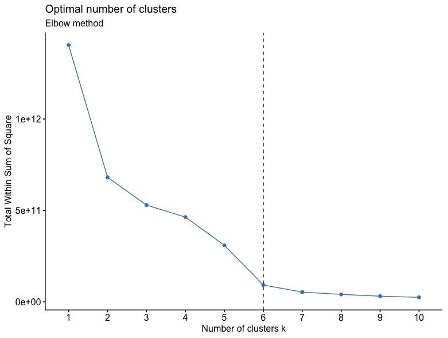
\includegraphics[width=0.4\textwidth]{Pengju/p-t-8.jpg}}
    \subfigure[]{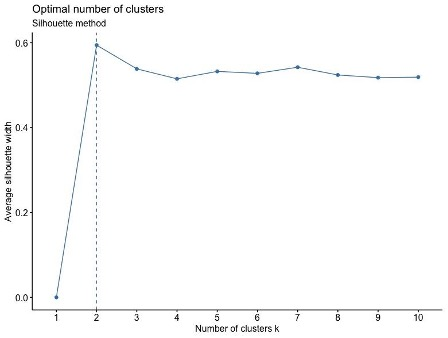
\includegraphics[width=0.4\textwidth]{Pengju/p-t-9.jpg}} 
    \caption{(a): Elbow Method  (b): Silhouette Method}
    \label{fig:foobar}
\end{figure}

\quad Lastly, we want to check if there is any better change with lower dimension, so we used principal component analysis for reducing our dataset, and did the same step for finding optimal clusters. We can see the cluster number change to 6 in this case, even though the silhouette plot gives 2 as well but it performs much better than the first one. 

\begin{figure}[H]
    \centering
    \subfigure[]{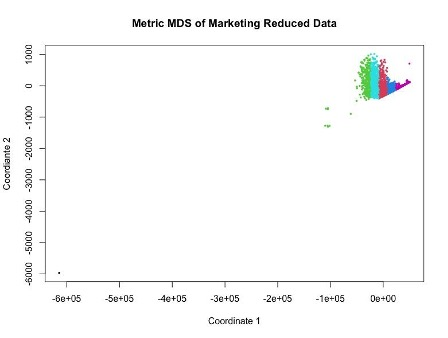
\includegraphics[width=0.4\textwidth]{Pengju/p-t-10.jpg}}
    \subfigure[]{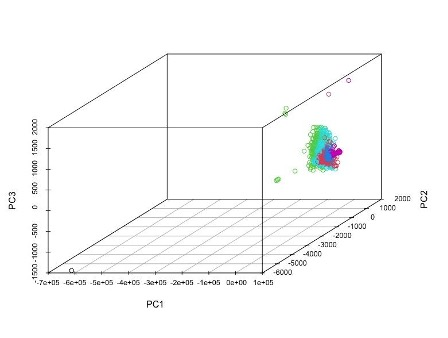
\includegraphics[width=0.4\textwidth]{Pengju/p-t-11.jpg}} 
    \caption{(a): Cluster of 6 in 2D (b): Cluster of 6 in 3D}
    \label{fig:foobar}
\end{figure}

\quad Reduced dataset models still have not enough separation, thus we conclude that maybe there are too many datasets, especially from different countries, that have no correlation between each other. 
\newpage
\section{Appendix}
% Isabelle Na Young Choi
\subsection{Isabelle Na Young Choi (Data Exploratory)}
\begin{itemize}
\item \textbf{Initial Regression}
\newline
I created two initial regressions using all variables and found a relationship between variables. There are two parts divided into groups which is a relationship between the total number of purchased variables and other features which are included in age, income, total children, recency, and amount of purchased products. And another initial regression is related to campaigns. This regression shows the response of a campaign variable with other campaign variables.
\item \textbf{Data Exploratory}
\newline
Before analyzing the marketing data, a data exploratory analysis process is necessary to find the best regression method and get better analysis results. The original marketing data is raw and unorganized so that it needs to preprocess to analyze clearly and precisely. Some variables have missing data and extensive data. Data cleaning process is necessary to perform the preprocessing process. We created some variables by merging data and dividing into groups. Next the initial regression shows strengths of relationship between variables. After checking the F-test, T-test, and the R-squared, we understand a relationship between the total\_num\_purchase variable and other variables. The last exploratory is the visualization relationships. We can see the relationship between numeric features and categorical features using a correlation matrix, box plot, and mosaic plot.
\item \textbf{Regression Analysis}
\newline
I created some regression models with the total number of purchases. According to the initial regression, I created an interaction model which is included in the total amount of variables. Also, I created lasso, ridge, and elastic net regression.
\item \textbf{Takeaway}
\newline
My main takeaway in this project is investigating this data and showing the relationship between variables before analyzing the dataset. The preprocessing phase is an important process to get better analysis and find a pathway of analysis. My responsibility is to represent preprocessing data processes and show initial regression and visualization. These processes interpret the data to investigate 4 different analyses of the marketing dataset. In the analysis process, we performed 4 different analyses, regression analysis, PCA, LDA, and clustering analysis. As we create different analyses and get results from them, it is a little bit hard to get simple and clear outcomes from the real data. Also, according to various analysis methods, we can get various results from the data. This project is a little bit of a long journey, but very interesting. 
\end{itemize}

% Stephanie Olivera
\subsection{Stephanie Olivera (Regression Analysis)}
For this project, I had two primary roles. My first role was to create initial visualizations for Milestone 3 to explore the data set prior to performing our different lines of analysis. My second role was to build, evaluate and interpret various regression models.
\begin{itemize}
\item \textbf{Data Visualization}
\newline
I created various visualizations to try to identify interesting relationships and parameters of interest in the dataset. I first created a pairwise correlation matrix to explore the relationships between all numeric features in the dataset. Here, I found two potential parameters of interest: total\_num\_purchase and total\_amount. Next, I created various box plots to see how the categorical features in the dataset are related to the total\_amount feature. Here, I found that income\_class, complain and response had the greatest variation of total\_amount based on class. Finally, I created multiple mosaic plots that show the relationship between the response feature and the categorical features age\_class, marital\_status, education and country. 
\item \textbf{Regression Analysis}
\newline
\textbf{OLS Regression}: For the regression analysis, I split the data into a 90\% train set and 10\% test set that would be used to evaluate the models. I then tried to fit an OLS model with all of the features that are acceptable for regression. Here, I found that only a few features were identified as significant and decided to proceed with all-subsets regression to find the optimal feature set. Here, I identified 9 significant features, retrained the model with this subset of features on the train set and evaluated its predictive performance on the test set. I found that the test RMSE was 25\% larger than the train RMSE, suggesting overfitting and potential benefit from regularization. Additionally, I calculated the VIF score for all of these features and found that they all had a value less than three. 
\newline
\textbf{Lasso Regression}: Next, I proceeded with Lasso and relaxed-Lasso regression to get independent evidence for obtaining features of interest. To create these models, I first plotted the mean-squared error against the log lambda to find the optimal lambda (and gamma in relaxed lasso) value. In both cases, I chose the lambda-1se value for the final lasso models. I found that regular and relaxed lasso selected almost the same features, with relaxed lasso dropping the teen\_home feature. I then compared the features selected here to the features selected in all-subsets regression above and found that they were very similar. The following features were selected by all models: Kidhome, MntFruits, MntMeatProducts, MntSweetProducts, MntGoldProducts and AcceptedCmp5. 
\newline
\textbf{Ridge Regression}: For the next model I chose to do Ridge regression to attempt to reduce the overfitting identified in the first OLS model. I again plotted the mean-squared error against the log-lambda value to obtain the optimal lambda value. I selected the lambda-1se value and retrained the regularized regression model on the train set. I then evaluated the predictions on the train and test sets and obtained a train RMSE of 3.7 and test RMSE of 4.37. Although there is still some overfitting, the test RMSE is now only 18\% larger than the train RMSE, compared to 25\% in the OLS regression model. 
\newline
\textbf{Elastic Net Regression}: For the final model I created an elastic net regression model that combined 50\% ridge and 50\% lasso to combine the good predictive performance of ridge and feature selection of lasso. Here, we were able to decrease the test RMSE compared to the lasso model, while keeping the feature selection capabilities of lasso. 
\item \textbf{Takeaway}
\newline
From the analysis that I have done so far, there are a few conclusions that can be drawn. First is that the following features are important for predicting the total\_num\_purchases: Kidhome, MntFruits, MntMeatProducts, MntSweetProducts, MntGoldProducts and AcceptedCmp5. The next takeaway is that Kidhome and AcceptedCmp5 have the largest impact on total\_num\_purchases. In terms of data analysis in general, I have learned that it’s important to try different values of parameters depending on the goal you have in mind. Here, I wanted to create more parsimonious models, so higher lambda values were preferred for regularization. I learned that when focusing on feature selection, it is important to try different approaches beyond all-subsets because they may not give the same exact result, as was the case here. Lastly, I learned that different approaches beyond regression and regularized-regression may be needed to make highly accurate predictions with noisy data.
\end{itemize}

% Milad Sabouri 
\subsection{Milad Sabouri (Principal Component Analysis)}
\begin{itemize}
\item \textbf{Overview}
\newline
In this project, we as a team tried to investigate a dataset that includes marketing data. In addition to data exploratory, we investigated four different parts of investigations including Regression with Regularization, Principal Component Analysis, Linear Discriminant Analysis, and Cluster Analysis. Based on our data exploratory analysis which we have submitted the results in Milestone 3, we found out that the data needs some modification in order to be suitable for further analysis. So, each group member took different responsibilities to deliver those types of preprocessing before we start our main analysis of the data.

\item \textbf{My Responsibility on The Team}
\newline
My responsibility on data exploratory analysis was investigating the data to see whether we can create new variables by merging some existing variables that will be important for later analyses. I have explained this part in more detail on the milestone-3 report. Also, as I mentioned earlier, our group is going to investigate 4 main analyses of the data. In Particular, I’m going to do Principal Component Analysis. My responsibility is to see how individual variables are related to each other and how we can provide a parsimonious model which enables us to interpret the data in a meaningful way without losing much information.

\item \textbf{Principal Component Analysis (PCA)}
\newline
After performing preprocessing on milestone 3, our dataset includes 22 numerical variables. By doing correlation analysis, I found out that some of the variables have different sorts of correlations. First, I performed a PCA analysis on the data to find how many components are significant. Since the data have different units, I set the scale parameter of prcomp to true in order to scale the data. I considered 4 different techniques (Cumulative Proportion, Knee on Scree Plot, VAR = 1, Parallel Analysis) to decide the appropriate number of factors. According to the cumulative proportion and var=1 techniques the number of factors should be 6. Also, according to parallel analysis and knee techniques the number of factors should be 4, so I tried both directions to see the results. I performed further PCA analysis by running the principal function. I tried to analyze rotating the components by using the VARIMAX option in the principal function. Also, I performed the PCA by running the factanal function to see whether there is any consensus on the results. Although the result of both principal and factanal functions were similar, neither 4 nor 6 components provided appropriate results that can be easily interpretable. Therefore, I decided to do some further analysis. First, by doing some cleaning factors analysis using corr.test function, I realized that two variables have almost no correlations with other variables. So, I excluded them from further PCA analysis. Moreover, I excluded variables that have correlations with more that 80\% of other variables. After that, I performed another PCA analysis to see how the results were changed.  Although the results were changed a little bit and the factors were clearer to interpret, still there were some ambiguities of interpretation. So, I decided to use the new variables that I have created in milestone 3. Hence, instead of using the TeenHome and KidHome variables, I created a new variable called NumChildren. Also, I aggregate all sorts of purchase types to one variable. I performed the PCA analysis again. Based on different techniques to select a number of factors, I came up with different numbers of factors. I decided to perform the PCA for each of those number of factors to see which one provides more clear results. In the end I came up with the final results which helped me to interpret the result in a meaningful way as much as possible. Also, the result of this analysis will help our team to do further analysis related to regression analysis and cluster analysis. According to my final result, the most parsimonious model that we can create based on the data includes 3 main factors which cover around 60\% of the data. Here is the final formula for each factor:
There are three components that I named them:
\begin{enumerate}
    \item Income
    \item Children
    \item Age
\end{enumerate}
The following are the formulas that show the contributor of each component: 
\begin{enumerate}
    \item \textbf{RC1 (Income)} = .807*Income - .568*NumWebVisitsMonth – .429*total\_children + .914*total\_amount + .897*total\_num\_purchases + .506*total\_acceptance
    \item \textbf{RC2 (Children)} = .898*NumDealPurchases + .501*NumWebVisitMonths + \\ .680*total\_children
    \item \textbf{RC3 (Age)} = .620*Age + .473*Recency + .544*Complain
\end{enumerate}
According to the results, income, total amount of purchases, total number of purchased items, and total number of acceptance of previous campaigns have positive contributions to the first factor which I named it Income because it has the most significant contributor of this factor. However, the number of web visits per month and total children at home have negative contributions to the first factor. On the other hand, the number of web visits and total children at home have positive contributions to the second factor which we named it Children. The contributors of the third factor are age, recency, and complaint. I named the third factor Age. The first factor (Income) shows us that income has an impact on total number of purchases and total amount of purchases while by increasing the number of children the total amount of purchase items may decrease. The Second factor (Children) shows us that households that have more children are more towards online shopping. It is because young people may like shopping in this way. Also, young people most like to shop for products that have discount deals. The third factor (Age) shows us that by increasing the age probably the number of complaints will increase as well.
\item \textbf{Takeaway}
\newline
My main takeaway from performing this project is how parsimonious models are important to enable us to have a clear interpretation of the data. To do that PCA is playing a critical role to create a parsimonious model. Also, I found out there is no single way to perform an analysis. We should perform different analyses with a different setup and then compare those results and look for consensus. To make this report fit in up to two pages, I only included some charts regarding my analysis.
\newpage
\begin{figure}
    \centering
    \subfigure[]{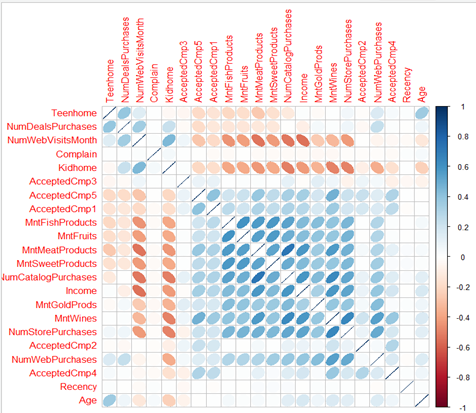
\includegraphics[width=0.4\textwidth]{Maild/m-t-1.png}}
    \subfigure[]{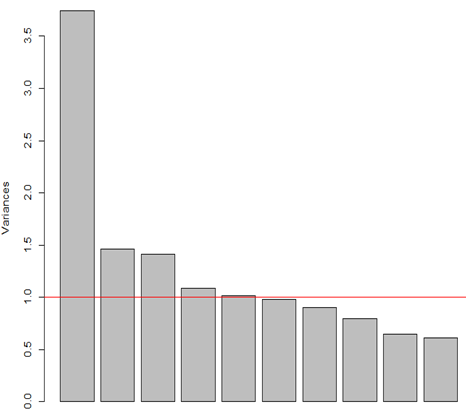
\includegraphics[width=0.4\textwidth]{Maild/m-t-2.png}} 
    \subfigure[]{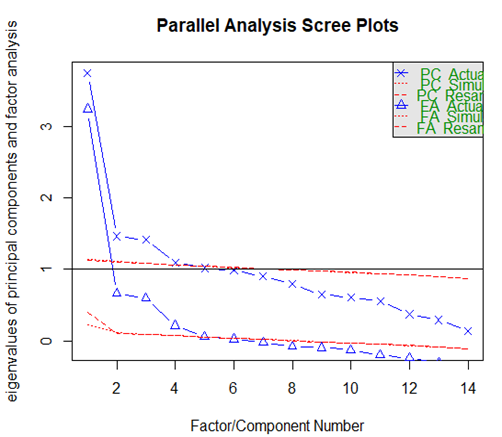
\includegraphics[width=0.4\textwidth]{Maild/m-t-3.png}}
    \subfigure[]{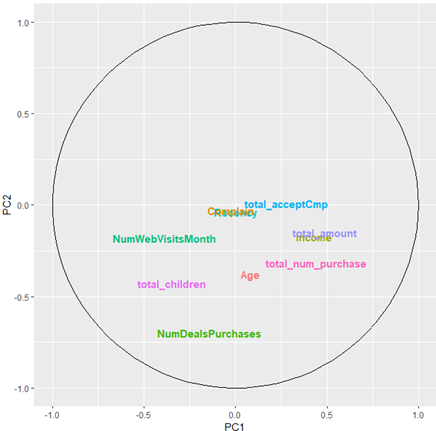
\includegraphics[width=0.4\textwidth]{Maild/m-t-4.png}}
    \caption{Maild's Analysis Charts}
    \label{fig:foobar}
\end{figure}
\end{itemize}

\subsection{Chien-Lin Yang (Linear Discriminant Analysis)}
\begin{itemize}
\item \textbf{Linear Discriminant Analysis (LDA)}
\newline
I am responsible for Linear Discriminant Analysis in this group of marketing data. Our data includes customer profiles, products purchased, campaign success (or failure), and channel performance. Also, the purpose is to predict whether customers will accept the marketing campaign based on the above data. The dependent variable is binary (yes/ no), and the independent variables are continuous, binary, and categorical variables.
\\
In the first part, since the dependent variable is binary, I use logistic regression analysis to compare with LDA. Besides, I use the confusion matrix and ROC curve to compare the performance of the two analyses. After running different training and test data many times, the performance of both is similar. In addition to understanding whether customers would accept the marketing campaign, I also want to find out if the consumer behavior and style could classify different income levels so that I could further target people in different income levels with an efficient approach to do different modes of a marketing campaign.
\\
In the second part, I use "income\_class" as the dependent variable, which has five levels: Poor, Lower-Middle, Middle, Upper-Middle, and Rich. The independent variables are different shopping styles, such as discount purchasing, catalog purchasing, store purchasing, and website purchasing. The initial model is difficult to see the classification of income levels, and the prediction accuracy is not good. I find that there is only one "Rich" observation in the income level. In the original data, the value is much larger than other observations, and it is also a weird number, 666,666. I guess this data should have some problems, but this one does not affect the overall 2,240 observations, so I change the data to be the "Upper-Middle" level. Also, I find that the "NumDealsPurchases" variable in the LD1 is less significant than the other variables, so I remove this variable. After adjusting both parts and running different training and test datasets, I find that the prediction accuracy becomes better, but the income level classification is still not easy to read. In summary, although the performance of classification is not good, LDA can give more insights and dimensionality reduction in the primary analysis.
\item \textbf{Takeaway}
\newline
In this course, I learned many different analyses and saw many examples. Before doing this final project, I thought I learned how to use the right analysis for the data, but that was not the case. It was only when I started doing the final project that I realized what real data was all about. First, I encounter a data cleaning problem in the beginning. I have to find ways to make the data clearer, but not to distort the original data. Then, I meet the poor performance of my analysis, and I have to try all kinds of adjustments and run all kinds of models to improve, and I probably do not end up with a significant improvement.
\\
Overall, when I was doing the final project, I realized what real data looks like and how data analysis is a long process. Also, poor performance is the normal situation in data analysis. What we have to do is try various ways and our domain knowledge to solve the problems, try to make the cold data into meaningful information, and finally provide a useful reference to the users. That process is hard but interesting.

\end{itemize}

\subsection{Pengju Zhang (Cluster Analysis)}
\begin{itemize}
\item \textbf{My Responsibility on The Team}
\newline
For analytical parts, my job is to clean the data and analyze our data through clustering. For non-technique parts, in order to keep all our contribution consistently, I used video editing to finalize our presentation and latex editor to format our final report.
\item \textbf{Data Cleaning}
\newline
I have converted the Date of Birth column to Age as a more reasonable variable, then convert Income from String type with useless “\$” to actual double value type, lastly replace all empty value with their corresponding mean value so it won’t affect our final result.
\item \textbf{Cluster Analysis}
\newline
Cluster analysis is a very interesting method of classification. It allows us to use unsupervised ways for self-classification by different algorithms, however unsupervised classification can lead to final results that are more difficult to interpret, especially when the clusters are relatively large.
\\
There are three parts that mainly affect the final result of the cluster analysis. The first is the number of clusters, which is also the most critical part. In our analysis, we chose dendrogram, elbow method and silhouette method as our reference. The second is the clustering algorithm, which requires several attempts to get satisfactory results, and we chose k-means for our model. Lastly is the choice of SEED, I chose 100 in my k-means algorithm for all both whole and reduced dataset to prevent the consistency, but I did not delve into this part.
\\
Finally is a conjecture about the results personally, we end up with a clear separation  in the k = 2 and k = 3 cases, but they are too concentrated leading to a very difficult interpretation. Although a clustering analysis with lower dimension yields better elbow and silhouette graphs, the final results are still too concentrated. I think this result is caused by too much data, and a better approach would be to first randomly select the data and divide it into a training and a test dataset, so that we can first reduce the amount of data and secondly avoid overfitting the results.
\item \textbf{Takeaway}
\newline
Multivariate analysis is a very complex subject, and what I learned from this course is not a single analytical method, but more about how to use these techniques to get a reasonable and explanatory model. I also learned that each technique needs to be mutually validated in order to have more accurate results, such as using PCA for dimensionality reduction in cluster analysis and using regularized regression to avoid overfitting.
\\
Last but not least, validation of the model by a domain expert is also essential. Although it is technically possible to obtain a reduced dimensional and accurate result, if there are unexplained factors in the model, it will be considered as a failed model.

\end{itemize}

\clearpage
%enter info to link bibtex file (.bib) in project
%\bibliography{example}   

%or enter each manually as below: 
\begin{thebibliography}{9}


\bibitem{githubLink}    
Jack Daoud. (2022, March). Marketing Analytics, Version 3. Retrieved January 30, 2022 from https://www.kaggle.com/jackdaoud/marketing-data.
\end{thebibliography}


\clearpage


\end{document} % The document ends here